
%\documentclass[a4paper]{jsbook}
%\usepackage{mcmd_jp}
%\begin{document}

\section{mmbucket 多次元均等化バケット分割\label{sect:mmbucket}}
\index{mmbucket@mmbucket}

\verb|f=|で指定した複数の数値項目を次元とした件数均等化バケット分割を行う。
例えば、\verb|f=a,b,c|そして\verb|n=5|と指定すると、
\hyperref[sect:mbucket]{mbucket}コマンドと同様に、項目\verb|a,b,c|それぞれを5つの区間に分割するが、
\verb|mmbucket|では、項目\verb|a,b,c|の3次元空間における各バケット(バケット数は$5^3=125$個になる)に
属する件数ができるだけ均等になるような区間を計算する

\subsection*{書式}
\verb|mmbucket f= n= [F=] [k=] [O=] [-ms] [-r]| 
\hyperref[sect:option_i]{[i=]}
\hyperref[sect:option_o]{[o=]}
\hyperref[sect:option_bufcount]{[bufcount=]} 
\hyperref[sect:option_assert_diffSize]{[-assert\_diffSize]}
\hyperref[sect:option_assert_nullkey]{[-assert\_nullkey]}
\hyperref[sect:option_assert_nullin]{[-assert\_nullin]}
\hyperref[sect:option_assert_nullout]{[-assert\_nullout]}
\hyperref[sect:option_nfn]{[-nfn]} 
\hyperref[sect:option_nfno]{[-nfno]}  
\hyperref[sect:option_x]{[-x]}
\hyperref[sect:option_q]{[-q]}
\hyperref[sect:option_option_tmppath]{[tmpPath=]}
\hyperref[sect:option_precision]{[precision=]}
\verb|[-params]|
\verb|[--help]|
\verb|[--helpl]|
\verb|[--version]|\\

\subsection*{パラメータ}
\begin{table}[hbt]
%\begin{center}
{\small
\begin{tabular}{ll}
\verb|i=|    & 入力ファイル名を指定する。\\
\verb|o=|    & 出力ファイル名を指定する。\\
\verb|f=|    & ここで指定した項目(複数項目指定可)の値を分割する。\\
             & 複数指定すれば、その数の次元に基づく均等化バケット分割を行う。\\
             & 1項目のみ指定すれば\verb|mbucket|と同じ結果になる。\\
             & \verb|-x,-nfn|オプション使用時は、項目番号(0〜)で指定可能。\\
\verb|n=|    & \verb|f=|で指定した項目数と同じ個数分指定する。\\
             & ただし1つの数字を指定した場合、\verb|f=|で指定した全ての項目に、同じ分割数が適用される。\\
\verb|F=|    & 出力形式を指定する。【デフォルト値:1】\\
             & バケットの名前を出力形式。\\
             & 0:バケット番号のみを表示する。\\
             & 1:バケットの範囲のみを表示する。\\
             & 2:バケット番号とバケット範囲の両方を表示する。\\
\verb|k=|    & バケット分割を行う単位となる項目名リスト(複数項目指定可)を指定する。\\
\verb|O=|    & \verb|f=|パラメータで指定した各項目の各バケットの数値範囲を出力するファイル名を指定する。\\
\verb|bufcount=| & バッファのサイズ数を指定する。 \\
\verb|-ms|   & 各項目を順次バケット分割していく時の開始項目を変えることで複数回のバケット分割をトライし、\\
             & よりよい解を求める。詳細は、以下の「アルゴリズムの概要」を参照のこと。\\
\verb|-r|    & バケット番号を逆順に出力する。\\
\end{tabular} 
}
\end{table} 

\subsection*{利用例}
\subsubsection*{Example 1: Basic Example}

Partition the number of records in column \verb|x,y| into two multi-dimentional equal subsets. At the same time, save the numeric range of each bucket in the file named \verb|rng.csv|.


\begin{Verbatim}[baselinestretch=0.7,frame=single]
$ more dat1.csv
id,x,y
A,2,7
B,6,7
C,5,6
D,7,5
E,6,4
F,1,3
G,3,3
H,4,2
I,7,2
J,2,1
$ mmbucket f=x:xb,y:yb n=2,2 O=rng.csv i=dat1.csv o=rsl1.csv
calculating on dimension ... #0 #1 done. VAR=30 updated!
calculating on dimension ... #0 #1 done. VAR=28 updated!
calculating on dimension ... #0 #1 done. VAR=28
#END# kgmbucket O=rng.csv f=x:xb,y:yb i=dat1.csv n=2,2 o=rsl1.csv
$ more rsl1.csv
id,x,y,xb,yb
A,2,7,1,2
B,6,7,2,2
C,5,6,2,2
D,7,5,2,2
E,6,4,2,1
F,1,3,1,1
G,3,3,1,1
H,4,2,2,1
I,7,2,2,1
J,2,1,1,1
$ more rng.csv
fieldName,bucketNo,rangeFrom,rangeTo
x,1,,3.5
x,2,3.5,
y,1,,4.5
y,2,4.5,
\end{Verbatim}
\subsubsection*{Example 2: Outupt Format}

Partition the number of records in column \verb|x,y| into two multi-dimentional equal subsets based on the \verb|id| field. The output format shall display the both the bucket number and numeric range.


\begin{Verbatim}[baselinestretch=0.7,frame=single]
$ more dat2.csv
id,x,y
A,2,7
A,6,7
A,5,6
B,7,5
B,6,4
B,1,3
C,3,3
C,4,2
C,7,2
C,2,1
$ mmbucket k=id f=x:xb,y:yb n=2,2 F=2 i=dat2.csv o=rsl2.csv
calculating on dimension ... #0 #1 done. VAR=3 updated!
calculating on dimension ... #0 #1 done. VAR=3
calculating on dimension ... #0 #1 done. VAR=3 updated!
calculating on dimension ... #0 #1 done. VAR=3
calculating on dimension ... #0 #1 done. VAR=6 updated!
calculating on dimension ... #0 #1 done. VAR=6
#END# kgmbucket F=2 f=x:xb,y:yb i=dat2.csv k=id n=2,2 o=rsl2.csv
$ more rsl2.csv
id%0,x,y,xb,yb
A,2,7,1:_3.5,2:6.5_
A,6,7,2:3.5_,2:6.5_
A,5,6,2:3.5_,1:_6.5
B,7,5,2:3.5_,2:4.5_
B,6,4,2:3.5_,1:_4.5
B,1,3,1:_3.5,1:_4.5
C,3,3,1:_3.5,2:1.5_
C,4,2,2:3.5_,2:1.5_
C,7,2,2:3.5_,2:1.5_
C,2,1,1:_3.5,1:_1.5
\end{Verbatim}

\subsection*{アルゴリズムの概要\footnote{このアルゴリズムは加藤直樹教授(京都大学工学研究科)による。}}

2つの数値項目からなるデータセット$D$があるものとし、2つの項目名を$A,B$とする。$A$および$B$の数値範囲をそれぞれ$K$個、$L$個に分割するものとする。この分割により、データセットは$K\cdot~L$個に分割される。mmbucketは分割された各領域(バケット)に入るデータの個数が一様になるような分割方法を求める。一様性の評価基準としては分散を用いるものとする。分散値が最小のバケット分割を求めるものであるが、ここでは、以下に述べるようなヒューリスティックスに基づいており、最適性は保証していない。アルゴリズムは以下のように記述される。\\
\\
1. 項目$A$について\hyperref[sect:mbucket]{件数均等化1次元バケット分割}をおこなう。\\
2. 1.で得られた$A$の分割を固定して、$B$の数値範囲のバケット分割をおこなう。このときの評価基準は2次元バケット分割の分散値である。方法は、件数均等化1次元バケット分割と同様に動的計画法を用いている。\\
3. 次にステップ2で得られたBの分割を固定して、$A$の数値範囲のバケット分割をおこなう。このときの評価基準はステップ2と同様に、2次元バケット分割の分散値である。\\
4. 以上のステップ2,3を分散値の改良が生じなくなるまで繰り返す。\\
5. 最終的に得られた分割を出力する。\\
\\
実装においては、ステップ1において、$A$と$B$の役割を入れ替えた場合も走らせて、解を求め、両者で得られた2つの解のうち優れた方を出力するようにしている。また、3次元以上の場合の均等化バケット分割も同様のアルゴリズムに基づいている。

\subsection*{mbucketとmmbucketの比較}

多次元バケット分割がどのように分割を行うかを示すために、1次元バケット分割との比較を通して以下で説明する。
表\ref{tbl:mmbucket_indata}には、二つの数値属性x,yを持つ、idがAからJまでの10件データが示されている。
このデータについて、属性x,yをそれぞれ2分割し計4つのバケットに分割することを考えよう。
属性xとyのそれぞれを1次元バケット分割することで得られた結果がx1,y1項目として示されており、
その値を用いて4つのバケットに分割した様子が図\label{fig:mmbucket_1dim}に示されている。
そして多次元バケット分割のアルゴリズムを用いて得られた結果がx2,y2項目として示されており、
その分割の様子が図\label{fig:mmbucket_2dim}に示されている。\\
分散値(各バケットに属するデータ件数の二乗和:詳しくは\hyperref[sect:mbucket]{mbucket}の定式化を参照)は、
1次元バケット分割においては、$Var_a'=1^2+4^2+4^2+1^2=34$となり、2次元バケット分割では$Var_b'=1^2+3^2+3^2+3^2=28$となる。
%また図1-(c)に示された分割の分散値も$Var_c'=2^2+2^2+4^2+2^2=28$で(b)の分割の分散値と等しい。
%このようなケースでは上記のアルゴリズムに示された繰り返しの過程で先に見つかった分割を優先する仕様となっている。\\
1次元バケット分割においては、x,yそれぞれ独立で考えた場合には、
分散を最小化する最適解となっている(すなわち5件ずつに分割している)が、
2次元の分割として評価すると、2次元バケット分割に比べて劣った分割となる。
このように多次元バケット分割を使うことで1次元バケット分割の組み合わせよりも優れた分割が可能となる。
しかしながら、次項で示すように、多次元分割はデータの内容によっては多大な計算時間が必要となるケースがあることに注意する。

\begin{table}[hbt]
\begin{center}
 \caption{サンプルデータとmbucket,mmbucketによる出力結果\label{tbl:mmbucket_indata}}
{\footnotesize
 \begin{tabular}{c|c|c|c|c|c|c}
  \hline
  \multicolumn{3}{c|}{データ} & \multicolumn{2}{|c|}{mbucket} & \multicolumn{2}{|c}{mmbucket} \\
\hline
id & x & y & x1 & y1 & x2 & y2 \\
\hline
A & 2 & 7 & 1 & 2 & 1 & 2 \\
B & 6 & 7 & 2 & 2 & 2 & 2 \\
C & 5 & 6 & 2 & 2 & 2 & 2 \\
D & 7 & 5 & 2 & 2 & 2 & 2 \\
E & 6 & 4 & 2 & 2 & 2 & 1 \\
F & 1 & 3 & 1 & 1 & 1 & 1 \\
G & 3 & 3 & 1 & 1 & 1 & 1 \\
H & 4 & 2 & 1 & 1 & 2 & 1 \\
I & 7 & 2 & 2 & 1 & 2 & 1 \\
J & 2 & 1& 1 & 1 & 1 & 1 \\ 
\hline
 \end{tabular}
}
\end{center}
\end{table}

\begin{figure}[htbp]
\begin{center}
\begin{tabular}{c}

\begin{minipage}{0.45\hsize}
\begin{center}
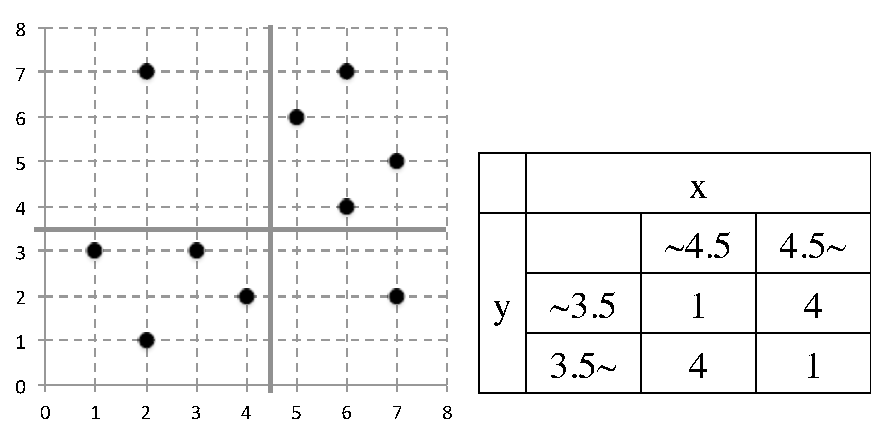
\includegraphics[scale=.50]{figure/mmbucket/split_mbucket.eps}
\end{center}
\caption{1次元分割(mbucket)×2による分割\label{fig:mmbucket_1dim}}
\end{minipage}

\begin{minipage}{0.45\hsize}
\begin{center}
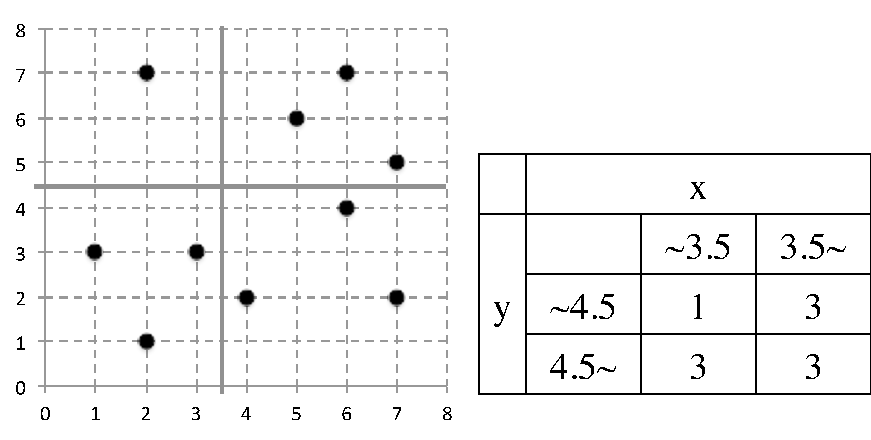
\includegraphics[scale=.50]{figure/mmbucket/split_mmbucket.eps}
\end{center}
\caption{2次元分割(mmbuket)による分割\label{fig:mmbucket_2dim}}
\end{minipage}

\end{tabular}
\end{center}
\end{figure}


%\begin{figure}[hbt]
%\begin{center}
%\includegraphics[width=20cm,bb=0 0 738 430]{./img/bucket_var.JPG}
%\caption{1次元分割×2による分割と2次元分割による分割の比較}
%\end{center}
%\end{figure}

\subsection*{多様な項目での精度実験}

mbucketとmmbucketの精度を実データを用いて比較してみる。
利用するデータは、エルニーニョ現象の解明を目的とした
\href{http://www.pmel.noaa.gov/tao/}{TAOプロジェクト}で収集されているデータで、
赤道付近に設置されたセンサーが収集した海洋データおよび気象データである。
表\ref{tbl:mmbucket_table1}にデータの一部を示す。\\

\begin{table}[hbt]
\begin{center}
\caption{精度実験用データセット\label{tbl:mmbucket_table0}}
{\footnotesize
%\begin{tabular}{p{2em}|p{2.5em}|p{2em}|p{3em}|p{3.5em}|p{4em}|p{4.5em}|p{4.5em}|p{3.5em}|p{3.5em}|p{4.5em}|p{2.5em}}\hline
\begin{tabular}{l|l|l|l|l|l|l|l|l|l|l|l}\hline
%obs  (観測id) & year (年)&month (月)&day (日)&date (日付) &latitude (緯度)&longitude (経度)&zonwinds (東西風速)	&merwinds (南北風速)&humidity (湿度)&air\_temp. (気温)&sstemp (海面温度) \\ \hline
id & year & month & day & date & latitude & longitude & zonwinds & merwinds & humidity & air\_temp. &sstemp \\ \hline
4060 & 93 &5 & 9 & 930509 & -0.02 & -109.96 & -2.1 & 2.1 & 81.2 & 26.8 & 27.02\\
4061 & 93 & 5 & 10 & 930510 & -0.02 & -109.96 & -3.4 & 1.4 & 84.2 & 26.95 & 26.91\\
4062 & 93 & 5 & 11 & 930511 & -0.02 & -109.96 & -3.8 & 2.2 & 84.9 & 26.98 & 26.78\\
4063 & 93 & 5 & 12 & 930512 & -0.02 & -109.96 & -3 & 1.5 & 86.9 & 26.93 & 26.74\\
4064 & 93 & 5 & 13 & 930513 & -0.02 & -109.96 & -4.5 & 1.9 & 87.6 & 27.01 & 26.82\\
4065 & 93 & 5 & 14 & 930514 & -0.02 & -109.96 & -5    & 1.3 & 85.6 & 26.96 & 26.68\\
\hline
\end{tabular}
\\
latitude:緯度, longitude:経度, zonwinds:東西風速, merwinds:南北風速, humidity:湿度, air\_temp.:気温, sstemp:海面温度
}
\end{center}
\end{table}

このデータの数値属性項目(緯度から海面温度までの7項目)を使いバケット分割の精度実験を行った。レコード行数は93,935行である。各項目の統計は表3に示す通りである。バケット分割においては「値の種類数」が計算時間に大きく影響を及ぼす。

\begin{table}[hbt]
\begin{center}
\caption{数値データの各種統計}
{\footnotesize
\begin{tabular}{c|c|c|c|c|c|c|c} \hline
計量& 緯度& 経度& 東西風速& 南北風速& 湿度& 気温& 海面温度\\ \hline
値の種類数& 482& 924& 228& 206& 385& 1104& 1201\\
算術平均& 0.305& -70.8& -3.35& -0.046& 81.3& 27.1& 27.9\\
標準偏差& 4.77& 128.7& 3.42& 3.021& 5.28& 1.674& 1.87\\
最小値& -8.33& -180& -10.7& -10.6& 52.1& 17.5& 18.2\\
中央値& 0.01& -125& -4.1& -0.1& 81.3& 27.5& 28.4\\
最大値& 9.05& 170.0& 14.3& 13& 99.9& 31.5& 31.0\\ \hline
\end{tabular}
}
\end{center}
\end{table}

7つの属性から2項目の組み合わせ全21通りについて1次元バケット分割(mbucket)に基づく方法と
2次元バケット分割(mmbucket)に基づく方法の分散値(バケットに属する件数の二乗和)の比較が
表\ref{tbl:mmbucket_table1}に示されている。
例えば一行目に示された結果は、気温×湿度のバケット分割の比較で、
mbucketでの分散値が408274409、mmbucketでの分散値が406438211であり、
その比(mmbucket/mbucket)が0.996であることが示されている。
続いて、分割数を10×10、15×15、20×20としたときの比が示されている。
結果は属性の組み合わせによって異なり、
「湿度×東西風速」のように全く改善の見られない属性の組み合わせもあれば、
「緯度×経度(15×15)」のように19\%(1-0.81)の精度向上を示す属性もみられる。
 
\begin{table}[hbt]
\begin{center}
\caption{mbucketとmmbucketによる2次元分割精度の比較\label{tbl:mmbucket_table1}}
{\footnotesize
\begin{tabular}{c|c||c|c|c|c|c|c}
\hline
% plastexにてmultirowはNG
%\multirow{2}{*}{項目1} & \multirow{2}{*}{項目2} & \multicolumn{2}{|c|}{分散値(5×5分割)} & \multicolumn{4}{|c}{分散値の比(mmbucket/mbucket)} \\  \cline{3-4}  \cline{5-8}
%                       &  & mbucket  & mmbucket & 5×5 &	10×10 & 15×15 & 20×20  \\ \hline\hline
            &          & \multicolumn{2}{|c|}{分散値(5×5分割)} & \multicolumn{4}{|c}{分散値の比(mmbucket/mbucket)} \\  \cline{3-4}  \cline{5-8}
項目1       & 項目2    & mbucket  & mmbucket & 5×5  &10×10 &15×15 & 20×20\\ \hline\hline
気温        & 湿度     &408274409 &406438211 &0.996 &0.987 &0.988 &0.981 \\
            & 緯度     &374125463 &371258775 &0.992 &0.988 &0.982 &0.964 \\
            & 経度     &490727955 &454663065 &0.927 &0.949 &0.946 &0.929 \\
            & 南北風速 &396436813 &394724219 &0.996 &0.991 &0.993 &0.989 \\
            & 海面温度 &816199131 &747215787 &0.915 &0.897 &0.883 &0.862 \\
            & 東西風速 &382069455 &381225143 &0.998 &0.998 &0.997 &0.996 \\  \hline
湿度        & 緯度     &368492959 &367941709 &0.999 &0.994 &0.994 &0.990 \\
            & 経度     &372116309 &370591351 &0.996 &0.991 &0.993 &0.986 \\
            & 南北風速 &355658757 &355658757 &1.000 &1.000 &1.000 &1.000 \\
            & 海面温度 &380382203 &379546293 &0.998 &0.991 &0.991 &0.983 \\
            & 東西風速 &357729819 &357697283 &1.000 &1.000 &1.000 &1.000 \\ \hline
緯度        & 経度     &365459223 &361754113 &0.990 &0.923 &0.812 &0.816 \\
            & 南北風速 &371478669 &370970251 &0.999 &0.988 &0.985 &0.982 \\
            & 海面温度 &392810425 &389589403 &0.992 &0.987 &0.979 &0.952 \\
            & 東西風速 &364521077 &364406663 &1.000 &0.999 &0.991 &0.992 \\ \hline
経度        & 南北風速 &414154185 &408431667 &0.986 &0.976 &0.976 &0.962 \\
            & 海面温度 &510979465 &463576537 &0.907 &0.945 &0.939 &0.934 \\
            & 東西風速 &400021527 &392710641 &0.982 &0.983 &0.982 &0.973 \\ \hline
南北風速    & 海面温度 &393233841 &392432943 &0.998 &0.995 &0.994 &0.993 \\
            & 東西風速 &359290669 &359074015 &0.999 &1.000 &1.000 &0.997 \\ \hline
海面温度    & 東西風速 &442877539 &438326669 &0.990 &0.988 &0.984 &0.986 \\ \hline
\end{tabular}
}
\end{center}
\end{table}
 
\subsection*{速度比較}

次に分割数による速度の違いみるための実験を行った。
前節と同様のデータを用い、気温×海面温度および緯度×経度について、
分割数を5から40まで5刻みで設定し、その実行時間を計測した。
その結果が表\ref{tbl:mmbucket_table2}に示されている。
mbucketの実行時間は分割数に関係なくほぼ一定である。
一方で2次元分割については分割数が多くなるに従って実行時間も長くなっている。
これはアルゴリズム内部で必要となる多次元直交数値範囲の選択において
効率的なアルゴリズムを実装していないためである。
これは改善可能であるが、次期バージョンでの課題としたい。


\begin{table}[hbt]
\begin{center}
\caption{サンプルデータとmbucket,mmbucketによる出力結果 \label{tbl:mmbucket_table2}}
{\footnotesize
\begin{tabular}{c|c|c|c|c}
\hline
& \multicolumn{2}{|c|}{気温×海面温度} & \multicolumn{2}{|c}{緯度×経度} \\ \hline
分割数 &mbucket &mmbucket &mbucket &mmbucket\\ \hline
5 &0.221 &2.21 &0.216 &0.67\\
10 &0.227 &3.90 &0.216 &1.67\\
15 &0.233 &10.4 &0.230 &3.28\\
20 &0.231 &26.1 &0.228 &7.13\\
25 &0.232 &32.9 &0.237 &13.3\\
30 &0.236 &46.7 &0.236 &11.4\\
35 &0.237 &62.3 &0.240 &15.2\\
40 &0.237 &80.1 &0.237 &25.8\\ \hline
\end{tabular}
}
\end{center}
\end{table}

\subsection*{関連コマンド}
\hyperref[sect:mbucket]{mbucket} : 複数項目指定しても、それぞれの項目で1次元バケット分割を実行する。

%\end{document}

%\fi
